\section{Datenmodell}
\setauthor{Hain Lukas}

\begin{figure}[H]
    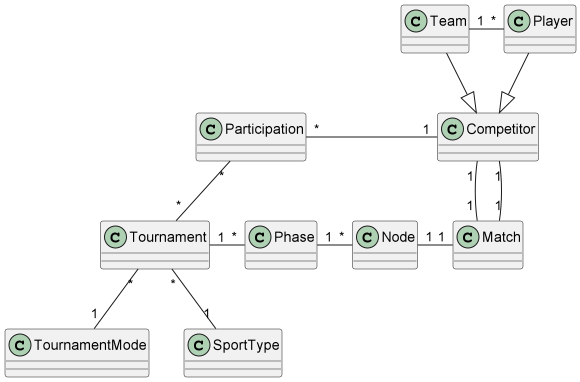
\includegraphics[scale=1]{pics/class_diagram.png}
    \caption{Class Diagram}
\end{figure}

Oben abgebildet ist das Datenmodell des Quarkus Backends. Anfangs erstellt man ein Turnier (Tournament), neben Namen, Startdatum und Enddatum 
wird hier noch der Turniermodus (TournamentMode) und die Sportart (SportType) festgelegt. Nun gibt man an, welche Teilnehmer (Competitor) an diesem Turnier teilnehmen (Participation). 
Ein Competitor kann entweder ein einzelner Spieler (Player) oder ein Team von Spielern (Team) sein.
Wenn das Turnier gestartet wird, wird das Turnier in Phasen (Phase) unterteilt. In jeder Phase gibt es eine bestimmte Anzahl an Matches (Match), welche jeweils 2 Competitor haben und mithilfe von Nodes (Node) 
der jeweiligen Phase zugeordnet werden.

\section{Quarkus Backend}
\setauthor{Hain Lukas}

\begin{figure}[H]
    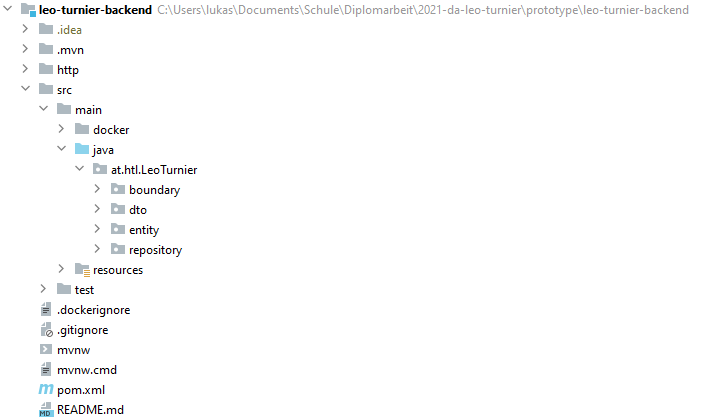
\includegraphics[scale=0.8]{pics/quarkus_file_structure.png}
    \caption{Quarkus Ordnerstruktur}
\end{figure}

(Ist dieser Teil zu Basic?)

Nach dem erstellen eines Quarkus Projektes ist ein Großteil der Ordnerstruktur bereits im vorhinein gegeben. Das wichtigste File im Projekt befindet sich ganz im äußersten Ordner, nämlich das "pom.xml" File. Hier werden 
nicht nur die Metadaten des Projekts angegeben, sondern auch die Dependencies, also alle externen Libraries, die die Applikation benötigt. 
Im "src" Ordner befinden sich ein "main" und ein "test" Ordner. Im "main" Ordner befindet sich der ganze Quellcode der Applikation, und im "test" Ordner befindet sich der Code, der den Quellcode auf seine richtigkeit prüft.
Im "main" Ordner befindet sich nun ein "docker" Ordner, auf den später noch eingegangen wird, ein "java" Ordner, in dem sich die Java Klassen der Applikation befindet, und ein "resources" Ordner, in dem weitere Files zu finden sind, 
auf die der Java Code eventuell zugreifen kann.

Die Java Klassen im "java" Ordner sind weiters in 4 verschiedene Ordner aufgeteilt. Im "entity" Ordner befinden sich alle Entitätsklassen der Applikation, also jene, die das Datenmodell (siehe Kapitel 6.1 Datenmodell) wiederspiegeln.
Die Klassen im "repository" sind die Schnittstelle zwischen der Quarkus Applikation und der Datenbank. Sie sind für die CRUD Operationen verantwortlich, also das Speichern, Auslesen, Verändern oder Löschen von Daten nach dem Schema der Entitätsklassen.
Außerdem befindet sich hier die Logik hinter den Turnieren. Die Klassen im "boundary" sind die Schnittstelle zum Frontend. Sie nehmen Requests, also Anforderungen, von außen an, 
führen die jeweilige Methode aus den Repository Klassen aus und liefern dann eine Response, also eine Antwort, zurück. Zuletzt gibt es noch die Klassen in "dto" Ordner, diese sind Klassen, in denen Daten gespeichert werden können, die für die Logik in den 
Repository Klassen benötigt wird, jedoch nicht unbedingt Teil des Datenmodells sind.

TODO: screenshot tournament

Oben abgebildet ist eine der Entitätsklassen dieser Applikation, nämlich die Tournament Klasse. Ganz oben, über der Klasse, ist die Annotation "@Entity" zu finden, um sicherzustellen, dass die Klasse von JPA als Entitätsklasse erkannt wird, und das Library dafür eine Tabelle erstellt.
Darunter befindet sich die "@Table" Annotation, die der Tabelle in der Datenbank ihren Namen gibt. Das Schema der Namensgebung von Tabellen lautet wie folgt: am Anfang steht immer die Abkürzung für den Tabellennamen, in diesem Fall ist das "T", danach kommt ein Unterstrich, 
gefolgt von dem Namen der Entitätsklasse in Großbuchstaben. In der Klasse selbst befinden sich nun die Klassenvariablen, welche von der Annotation "@Column" ihren Namen in der Datenbank verleiht. Das Schema der Namensgebung ist ähnlich, wie das der Tabellen: Anfangs die Abkürzung des Tabellennamens, 
dann ein Unterstrich als Trennung, gefolgt vom Namen der Klassenvariable, ebenfalls in Großbuchstaben. Die ID hat eine extra annotation, nämlich "@Id", das bedeutet dass sie der Primärschlüssel der Entitätsklasse ist. Außerdem steht bei den Variablen "tournamentmode" und "sportType" noch die "@ManyToOne" Annotation. 
Diese Felder werden dann in der Datenbank zu den Fremdschlüsseln auf andere Tabellen. Hier lautet das Namensschema wie folgt: Zuerst die Abkürzung der eigenen Klasse, dann der Name des Primärschlussels aus der Tabelle, auf die der Fremdschlüssel zeigt, wieder, getrennt durch einen Unterstrich.
Es gibt 4 Verschiedene Annotationen, die eine Beziehung zu anderen Tabellen herstellen:

\begin{itemize}
    \item @OneToOne
    \item @ManyToOne
    \item @OneToMany
    \item @ManyToMany
\end{itemize}

Die erste Mengenangabe steht immer für die eigene Klasse, die zweite steht für die andere Klasse. Diese braucht in diesem Fall natürlich auch die "@Entity" Annotation sowie einen Primärschlüssel. Bei "@OneToOne" und "@ManyToOne" wird in der Datenbank der Fremdschlüssel in der eigenen Tabelle erstellt, 
bei "@OneToMany" wird der Fremdschlüssel in der anderen Tabelle erstellt (hier muss die Variable, bei der die Annotation steht, auch eine Collection sein), und bei "@ManyToMany" wird eine Assotiationstabelle erstellt, in der sich dann 2 Fremdschlüssel befinden: 
einmal der au die Tabelle der eigenen Klasse, und einmal die der naderen Klasse.

Unter den Klassen befinden sich dann standardmäßig noch der Constructor sowie die Getter und Setter.
